\documentclass[1p]{elsarticle_modified}
%\bibliographystyle{elsarticle-num}

%\usepackage[colorlinks]{hyperref}
%\usepackage{abbrmath_seonhwa} %\Abb, \Ascr, \Acal ,\Abf, \Afrak
\usepackage{amsfonts}
\usepackage{amssymb}
\usepackage{amsmath}
\usepackage{amsthm}
\usepackage{scalefnt}
\usepackage{amsbsy}
\usepackage{kotex}
\usepackage{caption}
\usepackage{subfig}
\usepackage{color}
\usepackage{graphicx}
\usepackage{xcolor} %% white, black, red, green, blue, cyan, magenta, yellow
\usepackage{float}
\usepackage{setspace}
\usepackage{hyperref}

\usepackage{tikz}
\usetikzlibrary{arrows}

\usepackage{multirow}
\usepackage{array} % fixed length table
\usepackage{hhline}

%%%%%%%%%%%%%%%%%%%%%
\makeatletter
\renewcommand*\env@matrix[1][\arraystretch]{%
	\edef\arraystretch{#1}%
	\hskip -\arraycolsep
	\let\@ifnextchar\new@ifnextchar
	\array{*\c@MaxMatrixCols c}}
\makeatother %https://tex.stackexchange.com/questions/14071/how-can-i-increase-the-line-spacing-in-a-matrix
%%%%%%%%%%%%%%%

\usepackage[normalem]{ulem}

\newcommand{\msout}[1]{\ifmmode\text{\sout{\ensuremath{#1}}}\else\sout{#1}\fi}
%SOURCE: \msout is \stkout macro in https://tex.stackexchange.com/questions/20609/strikeout-in-math-mode

\newcommand{\cancel}[1]{
	\ifmmode
	{\color{red}\msout{#1}}
	\else
	{\color{red}\sout{#1}}
	\fi
}

\newcommand{\add}[1]{
	{\color{blue}\uwave{#1}}
}

\newcommand{\replace}[2]{
	\ifmmode
	{\color{red}\msout{#1}}{\color{blue}\uwave{#2}}
	\else
	{\color{red}\sout{#1}}{\color{blue}\uwave{#2}}
	\fi
}

\newcommand{\Sol}{\mathcal{S}} %segment
\newcommand{\D}{D} %diagram
\newcommand{\A}{\mathcal{A}} %arc


%%%%%%%%%%%%%%%%%%%%%%%%%%%%%5 test

\def\sl{\operatorname{\textup{SL}}(2,\Cbb)}
\def\psl{\operatorname{\textup{PSL}}(2,\Cbb)}
\def\quan{\mkern 1mu \triangleright \mkern 1mu}

\theoremstyle{definition}
\newtheorem{thm}{Theorem}[section]
\newtheorem{prop}[thm]{Proposition}
\newtheorem{lem}[thm]{Lemma}
\newtheorem{ques}[thm]{Question}
\newtheorem{cor}[thm]{Corollary}
\newtheorem{defn}[thm]{Definition}
\newtheorem{exam}[thm]{Example}
\newtheorem{rmk}[thm]{Remark}
\newtheorem{alg}[thm]{Algorithm}

\newcommand{\I}{\sqrt{-1}}
\begin{document}

%\begin{frontmatter}
%
%\title{Boundary parabolic representations of knots up to 8 crossings}
%
%%% Group authors per affiliation:
%\author{Yunhi Cho} 
%\address{Department of Mathematics, University of Seoul, Seoul, Korea}
%\ead{yhcho@uos.ac.kr}
%
%
%\author{Seonhwa Kim} %\fnref{s_kim}}
%\address{Center for Geometry and Physics, Institute for Basic Science, Pohang, 37673, Korea}
%\ead{ryeona17@ibs.re.kr}
%
%\author{Hyuk Kim}
%\address{Department of Mathematical Sciences, Seoul National University, Seoul 08826, Korea}
%\ead{hyukkim@snu.ac.kr}
%
%\author{Seokbeom Yoon}
%\address{Department of Mathematical Sciences, Seoul National University, Seoul, 08826,  Korea}
%\ead{sbyoon15@snu.ac.kr}
%
%\begin{abstract}
%We find all boundary parabolic representation of knots up to 8 crossings.
%
%\end{abstract}
%\begin{keyword}
%    \MSC[2010] 57M25 
%\end{keyword}
%
%\end{frontmatter}

%\linenumbers
%\tableofcontents
%
\newcommand\colored[1]{\textcolor{white}{\rule[-0.35ex]{0.8em}{1.4ex}}\kern-0.8em\color{red} #1}%
%\newcommand\colored[1]{\textcolor{white}{ #1}\kern-2.17ex	\textcolor{white}{ #1}\kern-1.81ex	\textcolor{white}{ #1}\kern-2.15ex\color{red}#1	}

{\Large $\underline{11a_{63}~(K11a_{63})}$}

\setlength{\tabcolsep}{10pt}
\renewcommand{\arraystretch}{1.6}
\vspace{1cm}\begin{tabular}{m{100pt}>{\centering\arraybackslash}m{274pt}}
\multirow{5}{120pt}{
	\centering
	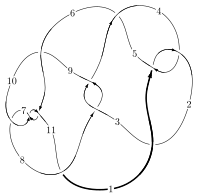
\includegraphics[width=112pt]{../../../GIT/diagram.site/Diagrams/png/312_11a_63.png}\\
\ \ \ A knot diagram\footnotemark}&
\allowdisplaybreaks
\textbf{Linearized knot diagam} \\
\cline{2-2}
 &
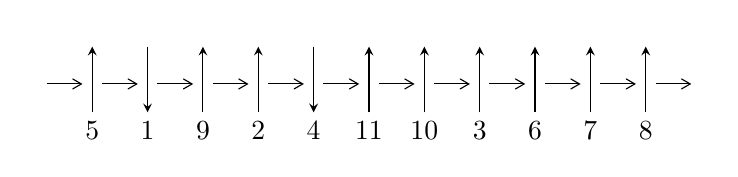
\begin{tikzpicture}[x=20pt, y=17pt]
	% nodes
	\node (C0) at (0, 0) {};
	\node (C1) at (1, 0) {};
	\node (C1U) at (1, +1) {};
	\node (C1D) at (1, -1) {5};

	\node (C2) at (2, 0) {};
	\node (C2U) at (2, +1) {};
	\node (C2D) at (2, -1) {1};

	\node (C3) at (3, 0) {};
	\node (C3U) at (3, +1) {};
	\node (C3D) at (3, -1) {9};

	\node (C4) at (4, 0) {};
	\node (C4U) at (4, +1) {};
	\node (C4D) at (4, -1) {2};

	\node (C5) at (5, 0) {};
	\node (C5U) at (5, +1) {};
	\node (C5D) at (5, -1) {4};

	\node (C6) at (6, 0) {};
	\node (C6U) at (6, +1) {};
	\node (C6D) at (6, -1) {11};

	\node (C7) at (7, 0) {};
	\node (C7U) at (7, +1) {};
	\node (C7D) at (7, -1) {10};

	\node (C8) at (8, 0) {};
	\node (C8U) at (8, +1) {};
	\node (C8D) at (8, -1) {3};

	\node (C9) at (9, 0) {};
	\node (C9U) at (9, +1) {};
	\node (C9D) at (9, -1) {6};

	\node (C10) at (10, 0) {};
	\node (C10U) at (10, +1) {};
	\node (C10D) at (10, -1) {7};

	\node (C11) at (11, 0) {};
	\node (C11U) at (11, +1) {};
	\node (C11D) at (11, -1) {8};
	\node (C12) at (12, 0) {};

	% arrows
	\draw[->,>={angle 60}]
	(C0) edge (C1) (C1) edge (C2) (C2) edge (C3) (C3) edge (C4) (C4) edge (C5) (C5) edge (C6) (C6) edge (C7) (C7) edge (C8) (C8) edge (C9) (C9) edge (C10) (C10) edge (C11) (C11) edge (C12) ;	\draw[->,>=stealth]
	(C1D) edge (C1U) (C2U) edge (C2D) (C3D) edge (C3U) (C4D) edge (C4U) (C5U) edge (C5D) (C6D) edge (C6U) (C7D) edge (C7U) (C8D) edge (C8U) (C9D) edge (C9U) (C10D) edge (C10U) (C11D) edge (C11U) ;
	\end{tikzpicture} \\
\hhline{~~} \\& 
\textbf{Solving Sequence} \\ \cline{2-2} 
 &
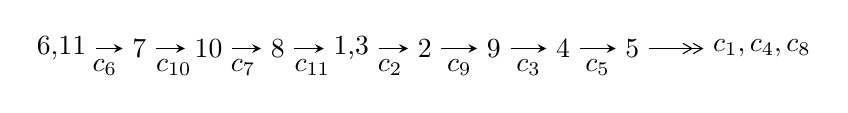
\begin{tikzpicture}[x=25pt, y=7pt]
	% node
	\node (A0) at (-1/8, 0) {6,11};
	\node (A1) at (1, 0) {7};
	\node (A2) at (2, 0) {10};
	\node (A3) at (3, 0) {8};
	\node (A4) at (65/16, 0) {1,3};
	\node (A5) at (41/8, 0) {2};
	\node (A6) at (49/8, 0) {9};
	\node (A7) at (57/8, 0) {4};
	\node (A8) at (65/8, 0) {5};
	\node (C1) at (1/2, -1) {$c_{6}$};
	\node (C2) at (3/2, -1) {$c_{10}$};
	\node (C3) at (5/2, -1) {$c_{7}$};
	\node (C4) at (7/2, -1) {$c_{11}$};
	\node (C5) at (37/8, -1) {$c_{2}$};
	\node (C6) at (45/8, -1) {$c_{9}$};
	\node (C7) at (53/8, -1) {$c_{3}$};
	\node (C8) at (61/8, -1) {$c_{5}$};
	\node (A9) at (10, 0) {$c_{1},c_{4},c_{8}$};

	% edge
	\draw[->,>=stealth]	
	(A0) edge (A1) (A1) edge (A2) (A2) edge (A3) (A3) edge (A4) (A4) edge (A5) (A5) edge (A6) (A6) edge (A7) (A7) edge (A8) ;
	\draw[->>,>={angle 60}]	
	(A8) edge (A9);
\end{tikzpicture} \\ 

\end{tabular} \\

\footnotetext{
The image of knot diagram is generated by the software ``\textbf{Draw programme}" developed by Andrew Bartholomew(\url{http://www.layer8.co.uk/maths/draw/index.htm\#Running-draw}), where we modified some parts for our purpose(\url{https://github.com/CATsTAILs/LinksPainter}).
}\phantom \\ \newline 
\centering \textbf{Ideals for irreducible components\footnotemark of $X_{\text{par}}$} 
 
\begin{align*}
I^u_{1}&=\langle 
7 u^{51}-22 u^{50}+\cdots+2 b+5,\;-5 u^{51}+8 u^{50}+\cdots+2 a+4,\;u^{52}-3 u^{51}+\cdots+3 u-1\rangle \\
I^u_{2}&=\langle 
- a u+b,\;- u^2 a+a^2- a u+2 u^2-2 a+u+3,\;u^3+u^2+2 u+1\rangle \\
\\
\end{align*}
\raggedright * 2 irreducible components of $\dim_{\mathbb{C}}=0$, with total 58 representations.\\
\footnotetext{All coefficients of polynomials are rational numbers. But the coefficients are sometimes approximated in decimal forms when there is not enough margin.}
\newpage
\renewcommand{\arraystretch}{1}
\centering \section*{I. $I^u_{1}= \langle 7 u^{51}-22 u^{50}+\cdots+2 b+5,\;-5 u^{51}+8 u^{50}+\cdots+2 a+4,\;u^{52}-3 u^{51}+\cdots+3 u-1 \rangle$}
\flushleft \textbf{(i) Arc colorings}\\
\begin{tabular}{m{7pt} m{180pt} m{7pt} m{180pt} }
\flushright $a_{6}=$&$\begin{pmatrix}1\\0\end{pmatrix}$ \\
\flushright $a_{11}=$&$\begin{pmatrix}0\\u\end{pmatrix}$ \\
\flushright $a_{7}=$&$\begin{pmatrix}1\\- u^2\end{pmatrix}$ \\
\flushright $a_{10}=$&$\begin{pmatrix}- u\\u^3+u\end{pmatrix}$ \\
\flushright $a_{8}=$&$\begin{pmatrix}u^2+1\\- u^4-2 u^2\end{pmatrix}$ \\
\flushright $a_{1}=$&$\begin{pmatrix}u^5+2 u^3+u\\- u^7-3 u^5-2 u^3+u\end{pmatrix}$ \\
\flushright $a_{3}=$&$\begin{pmatrix}\frac{5}{2} u^{51}-4 u^{50}+\cdots- u-2\\-\frac{7}{2} u^{51}+11 u^{50}+\cdots+\frac{19}{2} u-\frac{5}{2}\end{pmatrix}$ \\
\flushright $a_{2}=$&$\begin{pmatrix}u^{51}- u^{50}+\cdots+\frac{3}{2} u-\frac{5}{2}\\-\frac{3}{2} u^{51}+5 u^{50}+\cdots+\frac{11}{2} u-\frac{1}{2}\end{pmatrix}$ \\
\flushright $a_{9}=$&$\begin{pmatrix}- u^3-2 u\\u^3+u\end{pmatrix}$ \\
\flushright $a_{4}=$&$\begin{pmatrix}-\frac{3}{2} u^{51}+5 u^{50}+\cdots+5 u-5\\-\frac{1}{2} u^{51}+2 u^{50}+\cdots+\frac{5}{2} u+\frac{1}{2}\end{pmatrix}$ \\
\flushright $a_{5}=$&$\begin{pmatrix}\frac{1}{2} u^{51}- u^{50}+\cdots-6 u+1\\-\frac{1}{2} u^{51}+u^{50}+\cdots+\frac{3}{2} u-\frac{1}{2}\end{pmatrix}$\\ \flushright $a_{5}=$&$\begin{pmatrix}\frac{1}{2} u^{51}- u^{50}+\cdots-6 u+1\\-\frac{1}{2} u^{51}+u^{50}+\cdots+\frac{3}{2} u-\frac{1}{2}\end{pmatrix}$\\&\end{tabular}
\flushleft \textbf{(ii) Obstruction class $= -1$}\\~\\
\flushleft \textbf{(iii) Cusp Shapes $= 6 u^{51}-\frac{31}{2} u^{50}+\cdots-25 u+\frac{27}{2}$}\\~\\
\newpage\renewcommand{\arraystretch}{1}
\flushleft \textbf{(iv) u-Polynomials at the component}\newline \\
\begin{tabular}{m{50pt}|m{274pt}}
Crossings & \hspace{64pt}u-Polynomials at each crossing \\
\hline $$\begin{aligned}c_{1},c_{4}\end{aligned}$$&$\begin{aligned}
&u^{52}+4 u^{51}+\cdots-2 u+1
\end{aligned}$\\
\hline $$\begin{aligned}c_{2},c_{5}\end{aligned}$$&$\begin{aligned}
&u^{52}+16 u^{51}+\cdots-2 u+1
\end{aligned}$\\
\hline $$\begin{aligned}c_{3},c_{8}\end{aligned}$$&$\begin{aligned}
&u^{52}+u^{51}+\cdots-96 u-64
\end{aligned}$\\
\hline $$\begin{aligned}c_{6},c_{7},c_{10}\end{aligned}$$&$\begin{aligned}
&u^{52}+3 u^{51}+\cdots-3 u-1
\end{aligned}$\\
\hline $$\begin{aligned}c_{9},c_{11}\end{aligned}$$&$\begin{aligned}
&u^{52}-3 u^{51}+\cdots- u-34
\end{aligned}$\\
\hline
\end{tabular}\\~\\
\newpage\renewcommand{\arraystretch}{1}
\flushleft \textbf{(v) Riley Polynomials at the component}\newline \\
\begin{tabular}{m{50pt}|m{274pt}}
Crossings & \hspace{64pt}Riley Polynomials at each crossing \\
\hline $$\begin{aligned}c_{1},c_{4}\end{aligned}$$&$\begin{aligned}
&y^{52}+16 y^{51}+\cdots-2 y+1
\end{aligned}$\\
\hline $$\begin{aligned}c_{2},c_{5}\end{aligned}$$&$\begin{aligned}
&y^{52}+44 y^{51}+\cdots-286 y+1
\end{aligned}$\\
\hline $$\begin{aligned}c_{3},c_{8}\end{aligned}$$&$\begin{aligned}
&y^{52}-35 y^{51}+\cdots-21504 y+4096
\end{aligned}$\\
\hline $$\begin{aligned}c_{6},c_{7},c_{10}\end{aligned}$$&$\begin{aligned}
&y^{52}+43 y^{51}+\cdots-21 y+1
\end{aligned}$\\
\hline $$\begin{aligned}c_{9},c_{11}\end{aligned}$$&$\begin{aligned}
&y^{52}-41 y^{51}+\cdots-9793 y+1156
\end{aligned}$\\
\hline
\end{tabular}\\~\\
\newpage\flushleft \textbf{(vi) Complex Volumes and Cusp Shapes}
$$\begin{array}{c|c|c}  
\text{Solutions to }I^u_{1}& \I (\text{vol} + \sqrt{-1}CS) & \text{Cusp shape}\\
 \hline 
\begin{aligned}
u &= \phantom{-}0.869190 + 0.098347 I \\
a &= \phantom{-}2.62054 - 0.46093 I \\
b &= -2.32308 + 0.14292 I\end{aligned}
 & \phantom{-}10.69000 + 3.28668 I & \phantom{-}13.89309 - 1.28472 I \\ \hline\begin{aligned}
u &= \phantom{-}0.869190 - 0.098347 I \\
a &= \phantom{-}2.62054 + 0.46093 I \\
b &= -2.32308 - 0.14292 I\end{aligned}
 & \phantom{-}10.69000 - 3.28668 I & \phantom{-}13.89309 + 1.28472 I \\ \hline\begin{aligned}
u &= \phantom{-}0.863424 + 0.122136 I \\
a &= -2.58791 + 0.56862 I \\
b &= \phantom{-}2.30392 - 0.17488 I\end{aligned}
 & \phantom{-}9.82803 + 9.53725 I & \phantom{-}12.52453 - 6.18800 I \\ \hline\begin{aligned}
u &= \phantom{-}0.863424 - 0.122136 I \\
a &= -2.58791 - 0.56862 I \\
b &= \phantom{-}2.30392 + 0.17488 I\end{aligned}
 & \phantom{-}9.82803 - 9.53725 I & \phantom{-}12.52453 + 6.18800 I \\ \hline\begin{aligned}
u &= \phantom{-}0.824297\phantom{ +0.000000I} \\
a &= \phantom{-}2.98549\phantom{ +0.000000I} \\
b &= -2.46093\phantom{ +0.000000I}\end{aligned}
 & \phantom{-}6.31990\phantom{ +0.000000I} & \phantom{-}15.1000\phantom{ +0.000000I} \\ \hline\begin{aligned}
u &= -0.814922 + 0.019223 I \\
a &= -0.007593 - 0.403197 I \\
b &= -0.013938 - 0.328428 I\end{aligned}
 & \phantom{-}5.47556 - 2.92351 I & \phantom{-}12.21309 + 2.83301 I \\ \hline\begin{aligned}
u &= -0.814922 - 0.019223 I \\
a &= -0.007593 + 0.403197 I \\
b &= -0.013938 + 0.328428 I\end{aligned}
 & \phantom{-}5.47556 + 2.92351 I & \phantom{-}12.21309 - 2.83301 I \\ \hline\begin{aligned}
u &= -0.016991 + 1.193940 I \\
a &= -0.830637 + 0.202592 I \\
b &= \phantom{-}0.227769 + 0.995176 I\end{aligned}
 & -2.37385 - 1.42524 I & \phantom{-0.000000 } 0 \\ \hline\begin{aligned}
u &= -0.016991 - 1.193940 I \\
a &= -0.830637 - 0.202592 I \\
b &= \phantom{-}0.227769 - 0.995176 I\end{aligned}
 & -2.37385 + 1.42524 I & \phantom{-0.000000 } 0 \\ \hline\begin{aligned}
u &= \phantom{-}0.785467 + 0.056391 I \\
a &= -3.17951 + 0.44138 I \\
b &= \phantom{-}2.52229 - 0.16739 I\end{aligned}
 & \phantom{-}2.59377 + 3.74328 I & \phantom{-}10.41806 - 4.50899 I\\
 \hline 
 \end{array}$$\newpage$$\begin{array}{c|c|c}  
\text{Solutions to }I^u_{1}& \I (\text{vol} + \sqrt{-1}CS) & \text{Cusp shape}\\
 \hline 
\begin{aligned}
u &= \phantom{-}0.785467 - 0.056391 I \\
a &= -3.17951 - 0.44138 I \\
b &= \phantom{-}2.52229 + 0.16739 I\end{aligned}
 & \phantom{-}2.59377 - 3.74328 I & \phantom{-}10.41806 + 4.50899 I \\ \hline\begin{aligned}
u &= \phantom{-}0.429875 + 1.139080 I \\
a &= -1.01832 + 1.30146 I \\
b &= \phantom{-}1.92022 + 0.60048 I\end{aligned}
 & \phantom{-}6.71162 - 4.90299 I & \phantom{-0.000000 } 0 \\ \hline\begin{aligned}
u &= \phantom{-}0.429875 - 1.139080 I \\
a &= -1.01832 - 1.30146 I \\
b &= \phantom{-}1.92022 - 0.60048 I\end{aligned}
 & \phantom{-}6.71162 + 4.90299 I & \phantom{-0.000000 } 0 \\ \hline\begin{aligned}
u &= \phantom{-}0.429460 + 1.170320 I \\
a &= \phantom{-}1.00282 - 1.33702 I \\
b &= -1.99541 - 0.59942 I\end{aligned}
 & \phantom{-}7.39955 + 1.36157 I & \phantom{-0.000000 } 0 \\ \hline\begin{aligned}
u &= \phantom{-}0.429460 - 1.170320 I \\
a &= \phantom{-}1.00282 + 1.33702 I \\
b &= -1.99541 + 0.59942 I\end{aligned}
 & \phantom{-}7.39955 - 1.36157 I & \phantom{-0.000000 } 0 \\ \hline\begin{aligned}
u &= -0.536150 + 0.527494 I \\
a &= \phantom{-}0.081242 + 0.642665 I \\
b &= \phantom{-}0.382559 + 0.301710 I\end{aligned}
 & \phantom{-}4.30098 - 4.90907 I & \phantom{-}10.88602 + 6.29040 I \\ \hline\begin{aligned}
u &= -0.536150 - 0.527494 I \\
a &= \phantom{-}0.081242 - 0.642665 I \\
b &= \phantom{-}0.382559 - 0.301710 I\end{aligned}
 & \phantom{-}4.30098 + 4.90907 I & \phantom{-}10.88602 - 6.29040 I \\ \hline\begin{aligned}
u &= -0.571004 + 0.467263 I \\
a &= -0.110745 - 0.606288 I \\
b &= -0.346532 - 0.294446 I\end{aligned}
 & \phantom{-}4.49074 + 0.94301 I & \phantom{-}11.69221 + 0.65426 I \\ \hline\begin{aligned}
u &= -0.571004 - 0.467263 I \\
a &= -0.110745 + 0.606288 I \\
b &= -0.346532 + 0.294446 I\end{aligned}
 & \phantom{-}4.49074 - 0.94301 I & \phantom{-}11.69221 - 0.65426 I \\ \hline\begin{aligned}
u &= \phantom{-}0.054364 + 1.261730 I \\
a &= \phantom{-}1.155190 + 0.091004 I \\
b &= \phantom{-}0.05202 - 1.46248 I\end{aligned}
 & -3.61886 + 3.25992 I & \phantom{-0.000000 } 0\\
 \hline 
 \end{array}$$\newpage$$\begin{array}{c|c|c}  
\text{Solutions to }I^u_{1}& \I (\text{vol} + \sqrt{-1}CS) & \text{Cusp shape}\\
 \hline 
\begin{aligned}
u &= \phantom{-}0.054364 - 1.261730 I \\
a &= \phantom{-}1.155190 - 0.091004 I \\
b &= \phantom{-}0.05202 + 1.46248 I\end{aligned}
 & -3.61886 - 3.25992 I & \phantom{-0.000000 } 0 \\ \hline\begin{aligned}
u &= -0.192197 + 1.250340 I \\
a &= -0.288871 + 0.142351 I \\
b &= \phantom{-}0.122466 + 0.388546 I\end{aligned}
 & -2.79485 - 2.18309 I & \phantom{-0.000000 } 0 \\ \hline\begin{aligned}
u &= -0.192197 - 1.250340 I \\
a &= -0.288871 - 0.142351 I \\
b &= \phantom{-}0.122466 - 0.388546 I\end{aligned}
 & -2.79485 + 2.18309 I & \phantom{-0.000000 } 0 \\ \hline\begin{aligned}
u &= \phantom{-}0.327134 + 1.228210 I \\
a &= -1.20181 + 1.56811 I \\
b &= \phantom{-}2.31911 + 0.96309 I\end{aligned}
 & -0.998594 + 0.270066 I & \phantom{-0.000000 } 0 \\ \hline\begin{aligned}
u &= \phantom{-}0.327134 - 1.228210 I \\
a &= -1.20181 - 1.56811 I \\
b &= \phantom{-}2.31911 - 0.96309 I\end{aligned}
 & -0.998594 - 0.270066 I & \phantom{-0.000000 } 0 \\ \hline\begin{aligned}
u &= -0.361669 + 1.253070 I \\
a &= -0.116228 + 0.388450 I \\
b &= \phantom{-}0.444718 + 0.286131 I\end{aligned}
 & \phantom{-}1.65758 - 1.30987 I & \phantom{-0.000000 } 0 \\ \hline\begin{aligned}
u &= -0.361669 - 1.253070 I \\
a &= -0.116228 - 0.388450 I \\
b &= \phantom{-}0.444718 - 0.286131 I\end{aligned}
 & \phantom{-}1.65758 + 1.30987 I & \phantom{-0.000000 } 0 \\ \hline\begin{aligned}
u &= \phantom{-}0.369698 + 1.268120 I \\
a &= \phantom{-}0.96007 - 1.60608 I \\
b &= -2.39163 - 0.62372 I\end{aligned}
 & \phantom{-}2.38423 + 4.29256 I & \phantom{-0.000000 } 0 \\ \hline\begin{aligned}
u &= \phantom{-}0.369698 - 1.268120 I \\
a &= \phantom{-}0.96007 + 1.60608 I \\
b &= -2.39163 + 0.62372 I\end{aligned}
 & \phantom{-}2.38423 - 4.29256 I & \phantom{-0.000000 } 0 \\ \hline\begin{aligned}
u &= -0.362413 + 1.283420 I \\
a &= \phantom{-}0.090402 - 0.383341 I \\
b &= -0.459225 - 0.254952 I\end{aligned}
 & \phantom{-}1.42090 - 7.15944 I & \phantom{-0.000000 } 0\\
 \hline 
 \end{array}$$\newpage$$\begin{array}{c|c|c}  
\text{Solutions to }I^u_{1}& \I (\text{vol} + \sqrt{-1}CS) & \text{Cusp shape}\\
 \hline 
\begin{aligned}
u &= -0.362413 - 1.283420 I \\
a &= \phantom{-}0.090402 + 0.383341 I \\
b &= -0.459225 + 0.254952 I\end{aligned}
 & \phantom{-}1.42090 + 7.15944 I & \phantom{-0.000000 } 0 \\ \hline\begin{aligned}
u &= -0.046906 + 1.347120 I \\
a &= \phantom{-}0.608575 + 0.316639 I \\
b &= \phantom{-}0.455095 - 0.804970 I\end{aligned}
 & -6.61640 - 2.33196 I & \phantom{-0.000000 } 0 \\ \hline\begin{aligned}
u &= -0.046906 - 1.347120 I \\
a &= \phantom{-}0.608575 - 0.316639 I \\
b &= \phantom{-}0.455095 + 0.804970 I\end{aligned}
 & -6.61640 + 2.33196 I & \phantom{-0.000000 } 0 \\ \hline\begin{aligned}
u &= -0.639472 + 0.116337 I \\
a &= -0.129317 - 0.340252 I \\
b &= -0.122279 - 0.202537 I\end{aligned}
 & \phantom{-}0.592117 - 0.648848 I & \phantom{-}7.92572 + 0.14612 I \\ \hline\begin{aligned}
u &= -0.639472 - 0.116337 I \\
a &= -0.129317 + 0.340252 I \\
b &= -0.122279 + 0.202537 I\end{aligned}
 & \phantom{-}0.592117 + 0.648848 I & \phantom{-}7.92572 - 0.14612 I \\ \hline\begin{aligned}
u &= \phantom{-}0.344529 + 1.308900 I \\
a &= -0.84005 + 1.79324 I \\
b &= \phantom{-}2.63660 + 0.48172 I\end{aligned}
 & -1.67983 + 7.82276 I & \phantom{-0.000000 } 0 \\ \hline\begin{aligned}
u &= \phantom{-}0.344529 - 1.308900 I \\
a &= -0.84005 - 1.79324 I \\
b &= \phantom{-}2.63660 - 0.48172 I\end{aligned}
 & -1.67983 - 7.82276 I & \phantom{-0.000000 } 0 \\ \hline\begin{aligned}
u &= -0.266521 + 1.329970 I \\
a &= \phantom{-}0.007588 - 0.271037 I \\
b &= -0.358449 - 0.082329 I\end{aligned}
 & -3.96051 - 3.97418 I & \phantom{-0.000000 } 0 \\ \hline\begin{aligned}
u &= -0.266521 - 1.329970 I \\
a &= \phantom{-}0.007588 + 0.271037 I \\
b &= -0.358449 + 0.082329 I\end{aligned}
 & -3.96051 + 3.97418 I & \phantom{-0.000000 } 0 \\ \hline\begin{aligned}
u &= \phantom{-}0.389641 + 1.339870 I \\
a &= \phantom{-}0.68691 - 1.60534 I \\
b &= -2.41860 - 0.29487 I\end{aligned}
 & \phantom{-}6.17902 + 7.80504 I & \phantom{-0.000000 } 0\\
 \hline 
 \end{array}$$\newpage$$\begin{array}{c|c|c}  
\text{Solutions to }I^u_{1}& \I (\text{vol} + \sqrt{-1}CS) & \text{Cusp shape}\\
 \hline 
\begin{aligned}
u &= \phantom{-}0.389641 - 1.339870 I \\
a &= \phantom{-}0.68691 + 1.60534 I \\
b &= -2.41860 + 0.29487 I\end{aligned}
 & \phantom{-}6.17902 - 7.80504 I & \phantom{-0.000000 } 0 \\ \hline\begin{aligned}
u &= \phantom{-}0.381825 + 1.353460 I \\
a &= -0.63387 + 1.62633 I \\
b &= \phantom{-}2.44320 + 0.23695 I\end{aligned}
 & \phantom{-}5.1887 + 14.0116 I & \phantom{-0.000000 } 0 \\ \hline\begin{aligned}
u &= \phantom{-}0.381825 - 1.353460 I \\
a &= -0.63387 - 1.62633 I \\
b &= \phantom{-}2.44320 - 0.23695 I\end{aligned}
 & \phantom{-}5.1887 - 14.0116 I & \phantom{-0.000000 } 0 \\ \hline\begin{aligned}
u &= -0.16343 + 1.40977 I \\
a &= -0.251508 - 0.354319 I \\
b &= -0.540614 + 0.296661 I\end{aligned}
 & -1.50041 - 1.51719 I & \phantom{-0.000000 } 0 \\ \hline\begin{aligned}
u &= -0.16343 - 1.40977 I \\
a &= -0.251508 + 0.354319 I \\
b &= -0.540614 - 0.296661 I\end{aligned}
 & -1.50041 + 1.51719 I & \phantom{-0.000000 } 0 \\ \hline\begin{aligned}
u &= -0.12967 + 1.42233 I \\
a &= \phantom{-}0.311277 + 0.400831 I \\
b &= \phantom{-}0.610477 - 0.390766 I\end{aligned}
 & -1.95701 - 7.04982 I & \phantom{-0.000000 } 0 \\ \hline\begin{aligned}
u &= -0.12967 - 1.42233 I \\
a &= \phantom{-}0.311277 - 0.400831 I \\
b &= \phantom{-}0.610477 + 0.390766 I\end{aligned}
 & -1.95701 + 7.04982 I & \phantom{-0.000000 } 0 \\ \hline\begin{aligned}
u &= -0.134386 + 0.427009 I \\
a &= \phantom{-}0.202768 + 1.214100 I \\
b &= \phantom{-}0.545679 + 0.076573 I\end{aligned}
 & -1.24517 - 1.68566 I & \phantom{-}2.41923 + 5.81718 I \\ \hline\begin{aligned}
u &= -0.134386 - 0.427009 I \\
a &= \phantom{-}0.202768 - 1.214100 I \\
b &= \phantom{-}0.545679 - 0.076573 I\end{aligned}
 & -1.24517 + 1.68566 I & \phantom{-}2.41923 - 5.81718 I \\ \hline\begin{aligned}
u &= -0.364730\phantom{ +0.000000I} \\
a &= -0.713718\phantom{ +0.000000I} \\
b &= -0.260315\phantom{ +0.000000I}\end{aligned}
 & \phantom{-}0.683535\phantom{ +0.000000I} & \phantom{-}14.8020\phantom{ +0.000000I}\\
 \hline 
 \end{array}$$\newpage$$\begin{array}{c|c|c}  
\text{Solutions to }I^u_{1}& \I (\text{vol} + \sqrt{-1}CS) & \text{Cusp shape}\\
 \hline 
\begin{aligned}
u &= \phantom{-}0.261340 + 0.092384 I \\
a &= -0.16691 + 3.25412 I \\
b &= \phantom{-}0.344246 - 0.835011 I\end{aligned}
 & \phantom{-}0.38915 + 2.24131 I & \phantom{-}1.28116 - 4.34025 I \\ \hline\begin{aligned}
u &= \phantom{-}0.261340 - 0.092384 I \\
a &= -0.16691 - 3.25412 I \\
b &= \phantom{-}0.344246 + 0.835011 I\end{aligned}
 & \phantom{-}0.38915 - 2.24131 I & \phantom{-}1.28116 + 4.34025 I\\
 \hline 
 \end{array}$$\newpage\newpage\renewcommand{\arraystretch}{1}
\centering \section*{II. $I^u_{2}= \langle - a u+b,\;- u^2 a+a^2- a u+2 u^2-2 a+u+3,\;u^3+u^2+2 u+1 \rangle$}
\flushleft \textbf{(i) Arc colorings}\\
\begin{tabular}{m{7pt} m{180pt} m{7pt} m{180pt} }
\flushright $a_{6}=$&$\begin{pmatrix}1\\0\end{pmatrix}$ \\
\flushright $a_{11}=$&$\begin{pmatrix}0\\u\end{pmatrix}$ \\
\flushright $a_{7}=$&$\begin{pmatrix}1\\- u^2\end{pmatrix}$ \\
\flushright $a_{10}=$&$\begin{pmatrix}- u\\- u^2- u-1\end{pmatrix}$ \\
\flushright $a_{8}=$&$\begin{pmatrix}u^2+1\\- u^2- u-1\end{pmatrix}$ \\
\flushright $a_{1}=$&$\begin{pmatrix}-1\\0\end{pmatrix}$ \\
\flushright $a_{3}=$&$\begin{pmatrix}a\\a u\end{pmatrix}$ \\
\flushright $a_{2}=$&$\begin{pmatrix}a u+a\\a u\end{pmatrix}$ \\
\flushright $a_{9}=$&$\begin{pmatrix}u^2+1\\- u^2- u-1\end{pmatrix}$ \\
\flushright $a_{4}=$&$\begin{pmatrix}a\\a u\end{pmatrix}$ \\
\flushright $a_{5}=$&$\begin{pmatrix}- u^2+a- u-1\\a u+1\end{pmatrix}$\\ \flushright $a_{5}=$&$\begin{pmatrix}- u^2+a- u-1\\a u+1\end{pmatrix}$\\&\end{tabular}
\flushleft \textbf{(ii) Obstruction class $= 1$}\\~\\
\flushleft \textbf{(iii) Cusp Shapes $= u^2 a-4 a u+5 u^2- a+5 u+12$}\\~\\
\newpage\renewcommand{\arraystretch}{1}
\flushleft \textbf{(iv) u-Polynomials at the component}\newline \\
\begin{tabular}{m{50pt}|m{274pt}}
Crossings & \hspace{64pt}u-Polynomials at each crossing \\
\hline $$\begin{aligned}c_{1},c_{2},c_{5}\end{aligned}$$&$\begin{aligned}
&(u^2+u+1)^3
\end{aligned}$\\
\hline $$\begin{aligned}c_{3},c_{8}\end{aligned}$$&$\begin{aligned}
&u^6
\end{aligned}$\\
\hline $$\begin{aligned}c_{4}\end{aligned}$$&$\begin{aligned}
&(u^2- u+1)^3
\end{aligned}$\\
\hline $$\begin{aligned}c_{6},c_{7}\end{aligned}$$&$\begin{aligned}
&(u^3+u^2+2 u+1)^2
\end{aligned}$\\
\hline $$\begin{aligned}c_{9},c_{11}\end{aligned}$$&$\begin{aligned}
&(u^3+u^2-1)^2
\end{aligned}$\\
\hline $$\begin{aligned}c_{10}\end{aligned}$$&$\begin{aligned}
&(u^3- u^2+2 u-1)^2
\end{aligned}$\\
\hline
\end{tabular}\\~\\
\newpage\renewcommand{\arraystretch}{1}
\flushleft \textbf{(v) Riley Polynomials at the component}\newline \\
\begin{tabular}{m{50pt}|m{274pt}}
Crossings & \hspace{64pt}Riley Polynomials at each crossing \\
\hline $$\begin{aligned}c_{1},c_{2},c_{4}\\c_{5}\end{aligned}$$&$\begin{aligned}
&(y^2+y+1)^3
\end{aligned}$\\
\hline $$\begin{aligned}c_{3},c_{8}\end{aligned}$$&$\begin{aligned}
&y^6
\end{aligned}$\\
\hline $$\begin{aligned}c_{6},c_{7},c_{10}\end{aligned}$$&$\begin{aligned}
&(y^3+3 y^2+2 y-1)^2
\end{aligned}$\\
\hline $$\begin{aligned}c_{9},c_{11}\end{aligned}$$&$\begin{aligned}
&(y^3- y^2+2 y-1)^2
\end{aligned}$\\
\hline
\end{tabular}\\~\\
\newpage\flushleft \textbf{(vi) Complex Volumes and Cusp Shapes}
$$\begin{array}{c|c|c}  
\text{Solutions to }I^u_{2}& \I (\text{vol} + \sqrt{-1}CS) & \text{Cusp shape}\\
 \hline 
\begin{aligned}
u &= -0.215080 + 1.307140 I \\
a &= \phantom{-}0.706350 + 0.266290 I \\
b &= -0.500000 + 0.866025 I\end{aligned}
 & -3.02413 - 4.85801 I & \phantom{-}6.43615 + 6.24253 I \\ \hline\begin{aligned}
u &= -0.215080 + 1.307140 I \\
a &= -0.583789 + 0.478572 I \\
b &= -0.500000 - 0.866025 I\end{aligned}
 & -3.02413 - 0.79824 I & \phantom{-}2.88198 - 0.84592 I \\ \hline\begin{aligned}
u &= -0.215080 - 1.307140 I \\
a &= \phantom{-}0.706350 - 0.266290 I \\
b &= -0.500000 - 0.866025 I\end{aligned}
 & -3.02413 + 4.85801 I & \phantom{-}6.43615 - 6.24253 I \\ \hline\begin{aligned}
u &= -0.215080 - 1.307140 I \\
a &= -0.583789 - 0.478572 I \\
b &= -0.500000 + 0.866025 I\end{aligned}
 & -3.02413 + 0.79824 I & \phantom{-}2.88198 + 0.84592 I \\ \hline\begin{aligned}
u &= -0.569840\phantom{ +0.000000I} \\
a &= \phantom{-}0.87744 + 1.51977 I \\
b &= -0.500000 - 0.866025 I\end{aligned}
 & \phantom{-}1.11345 - 2.02988 I & \phantom{-}12.18187 + 2.43783 I \\ \hline\begin{aligned}
u &= -0.569840\phantom{ +0.000000I} \\
a &= \phantom{-}0.87744 - 1.51977 I \\
b &= -0.500000 + 0.866025 I\end{aligned}
 & \phantom{-}1.11345 + 2.02988 I & \phantom{-}12.18187 - 2.43783 I\\
 \hline 
 \end{array}$$\newpage
\newpage\renewcommand{\arraystretch}{1}
\centering \section*{ III. u-Polynomials}
\begin{tabular}{m{50pt}|m{274pt}}
Crossings & \hspace{64pt}u-Polynomials at each crossing \\
\hline $$\begin{aligned}c_{1}\end{aligned}$$&$\begin{aligned}
&((u^2+u+1)^3)(u^{52}+4 u^{51}+\cdots-2 u+1)
\end{aligned}$\\
\hline $$\begin{aligned}c_{2},c_{5}\end{aligned}$$&$\begin{aligned}
&((u^2+u+1)^3)(u^{52}+16 u^{51}+\cdots-2 u+1)
\end{aligned}$\\
\hline $$\begin{aligned}c_{3},c_{8}\end{aligned}$$&$\begin{aligned}
&u^6(u^{52}+u^{51}+\cdots-96 u-64)
\end{aligned}$\\
\hline $$\begin{aligned}c_{4}\end{aligned}$$&$\begin{aligned}
&((u^2- u+1)^3)(u^{52}+4 u^{51}+\cdots-2 u+1)
\end{aligned}$\\
\hline $$\begin{aligned}c_{6},c_{7}\end{aligned}$$&$\begin{aligned}
&((u^3+u^2+2 u+1)^2)(u^{52}+3 u^{51}+\cdots-3 u-1)
\end{aligned}$\\
\hline $$\begin{aligned}c_{9},c_{11}\end{aligned}$$&$\begin{aligned}
&((u^3+u^2-1)^2)(u^{52}-3 u^{51}+\cdots- u-34)
\end{aligned}$\\
\hline $$\begin{aligned}c_{10}\end{aligned}$$&$\begin{aligned}
&((u^3- u^2+2 u-1)^2)(u^{52}+3 u^{51}+\cdots-3 u-1)
\end{aligned}$\\
\hline
\end{tabular}\newpage\renewcommand{\arraystretch}{1}
\centering \section*{ IV. Riley Polynomials}
\begin{tabular}{m{50pt}|m{274pt}}
Crossings & \hspace{64pt}Riley Polynomials at each crossing \\
\hline $$\begin{aligned}c_{1},c_{4}\end{aligned}$$&$\begin{aligned}
&((y^2+y+1)^3)(y^{52}+16 y^{51}+\cdots-2 y+1)
\end{aligned}$\\
\hline $$\begin{aligned}c_{2},c_{5}\end{aligned}$$&$\begin{aligned}
&((y^2+y+1)^3)(y^{52}+44 y^{51}+\cdots-286 y+1)
\end{aligned}$\\
\hline $$\begin{aligned}c_{3},c_{8}\end{aligned}$$&$\begin{aligned}
&y^6(y^{52}-35 y^{51}+\cdots-21504 y+4096)
\end{aligned}$\\
\hline $$\begin{aligned}c_{6},c_{7},c_{10}\end{aligned}$$&$\begin{aligned}
&((y^3+3 y^2+2 y-1)^2)(y^{52}+43 y^{51}+\cdots-21 y+1)
\end{aligned}$\\
\hline $$\begin{aligned}c_{9},c_{11}\end{aligned}$$&$\begin{aligned}
&((y^3- y^2+2 y-1)^2)(y^{52}-41 y^{51}+\cdots-9793 y+1156)
\end{aligned}$\\
\hline
\end{tabular}
\vskip 2pc
\end{document}